% !BIB TS-program = biber

\RequirePackage[l2tabu,orthodox]{nag}

% TODO: decide if one-sided/two-sided
%\documentclass[headsepline,footsepline,footinclude=false,fontsize=11pt,paper=a4,listof=totoc,bibliography=totoc,BCOR=12mm,DIV=12]{scrbook} % two-sided
\documentclass[headsepline,footsepline,footinclude=false,oneside,fontsize=11pt,paper=a4,listof=totoc,bibliography=totoc]{scrbook} % one-sided

% TODO: change citation style in settings
\PassOptionsToPackage{table,svgnames,dvipsnames}{xcolor}

\usepackage[utf8]{inputenc}
\usepackage[T1]{fontenc}
\usepackage[sc]{mathpazo}
\usepackage[ngerman,american]{babel}
\usepackage[autostyle]{csquotes}
\usepackage[%
  backend=biber,
  url=false,
  style=alphabetic,
  maxnames=4,
  minnames=3,
  maxbibnames=99,
  giveninits,
  uniquename=init]{biblatex} % TODO: adapt citation style
\usepackage{graphicx}
\usepackage{scrhack} % necessary for listings package
\usepackage{listings}
\usepackage{lstautogobble}
\usepackage{tikz}
\usepackage{pgfplots}
\usepackage{pgfplotstable}
\usepackage{booktabs}
\usepackage[final]{microtype}
\usepackage{caption}
\usepackage[printonlyused]{acronym}
\usepackage[hidelinks]{hyperref} % hidelinks removes colored boxes around references and links
\AtBeginDocument{%
	\hypersetup{
		pdftitle=\getTitle,
		pdfauthor=\getAuthor,
	}
}
\usepackage{ifthen}

% for fachschaft_print.pdf
\makeatletter
\if@twoside{}
	\typeout{TUM-Dev LaTeX-Thesis-Template: twoside}
\else
	\typeout{TUM-Dev LaTeX-Thesis-Template: oneside}
\fi
\makeatother

\addto\extrasamerican{
	\def\lstnumberautorefname{Line}
	\def\chapterautorefname{Chapter}
	\def\sectionautorefname{Section}
	\def\subsectionautorefname{Subsection}
	\def\subsubsectionautorefname{Subsubsection}
}

\addto\extrasngerman{
	\def\lstnumberautorefname{Zeile}
}

% Themes
\ifthenelse{\equal{\detokenize{dark}}{\jobname}}{%
  % Dark theme
  \newcommand{\bg}{black} % background
  \newcommand{\fg}{white} % foreground
  \usepackage[pagecolor=\bg]{pagecolor}
  \color{\fg}
}{%
  % Light theme
  \newcommand{\bg}{white} % background
  \newcommand{\fg}{black} % foreground
}

\bibliography{bibliography}

\setkomafont{disposition}{\normalfont\bfseries} % use serif font for headings
\linespread{1.05} % adjust line spread for mathpazo font

% Add table of contents to PDF bookmarks
\BeforeTOCHead[toc]{{\cleardoublepage\pdfbookmark[0]{\contentsname}{toc}}}

% Define TUM corporate design colors
% Taken from http://portal.mytum.de/corporatedesign/index_print/vorlagen/index_farben
\definecolor{TUMBlue}{HTML}{0065BD}
\definecolor{TUMSecondaryBlue}{HTML}{005293}
\definecolor{TUMSecondaryBlue2}{HTML}{003359}
\definecolor{TUMBlack}{HTML}{000000}
\definecolor{TUMWhite}{HTML}{FFFFFF}
\definecolor{TUMDarkGray}{HTML}{333333}
\definecolor{TUMGray}{HTML}{808080}
\definecolor{TUMLightGray}{HTML}{CCCCC6}
\definecolor{TUMAccentGray}{HTML}{DAD7CB}
\definecolor{TUMAccentOrange}{HTML}{E37222}
\definecolor{TUMAccentGreen}{HTML}{A2AD00}
\definecolor{TUMAccentLightBlue}{HTML}{98C6EA}
\definecolor{TUMAccentBlue}{HTML}{64A0C8}

% Settings for pgfplots
\pgfplotsset{compat=newest}
\pgfplotsset{
  % For available color names, see http://www.latextemplates.com/svgnames-colors
  cycle list={TUMBlue\\TUMAccentOrange\\TUMAccentGreen\\TUMSecondaryBlue2\\TUMDarkGray\\},
}

% Settings for lstlistings
\lstset{%
  basicstyle=\ttfamily,
  columns=fullflexible,
  autogobble,
  keywordstyle=\bfseries\color{TUMBlue},
  stringstyle=\color{TUMAccentGreen},
  captionpos=b
}


% TODO: change thesis information
\newcommand*{\getUniversity}{Technische Universität München}
\newcommand*{\getFaculty}{Informatics}
\newcommand*{\getDegree}{Data Engineering and Analytics}
\newcommand*{\getSchool}{Computation, Information and Technology}
\newcommand*{\getTitle}{Enhancing Software Fuzzing through Dynamic Instrumentation}
\newcommand*{\getTitleGer}{Verbesserung des Software-Fuzzings durch dynamische Instrumentierung}
\newcommand*{\getAuthor}{Cosmin Banica}
\newcommand*{\getDoctype}{Master's Thesis}
\newcommand*{\getSupervisor}{Supervisor}
\newcommand*{\getAdvisor}{Advisor}
\newcommand*{\getSubmissionDate}{15.01.2024}
\newcommand*{\getSubmissionLocation}{Munich}

\begin{document}

% Set page numbering to avoid "destination with the same identifier has been already used" warning for cover page.
% (see https://en.wikibooks.org/wiki/LaTeX/Hyperlinks#Problems_with_Links_and_Pages).
\pagenumbering{alph}
\begin{titlepage}
  % HACK for two-sided documents: ignore binding correction for cover page.
  % Adapted from Markus Kohm's KOMA-Script titlepage=firstiscover handling.
  % See http://mirrors.ctan.org/macros/latex/contrib/koma-script/scrkernel-title.dtx,
  % \maketitle macro.
  \oddsidemargin=\evensidemargin\relax
  \textwidth=\dimexpr\paperwidth-2\evensidemargin-2in\relax
  \hsize=\textwidth\relax

  \centering

  \IfFileExists{logos/tum.pdf}{%
    \includegraphics[height=20mm]{logos/tum.pdf}
  }{%
    \vspace*{20mm}
  }

  \vspace{5mm}
  {\huge\MakeUppercase{School of \getSchool{} --- \getFaculty{}} \par}

  \vspace{5mm}
  {\large\MakeUppercase{\getUniversity{}} \par}

  \vspace{15mm}
  {\Large \getDoctype{} in \getDegree{} \par}

  \vspace{10mm}
  {\huge\bfseries \getTitle{} \par}

  \vspace{10mm}
  {\LARGE \getAuthor{}}

  \IfFileExists{logos/faculty.png}{%
    \vfill{}
    
\includegraphics[height=20mm]{logos/faculty.png}
  }{}
\end{titlepage}


\frontmatter{}

\begin{titlepage}
  \centering

  \IfFileExists{logos/tum.pdf}{%
    \includegraphics[height=20mm]{logos/tum.pdf}
  }{%
    \vspace*{20mm}
  }

  \vspace{5mm}
  {\huge\MakeUppercase{School of \getSchool{} --- \getFaculty{}} \par}

  \vspace{5mm}
  {\large\MakeUppercase{\getUniversity{}} \par}

  \vspace{20mm}
  {\Large \getDoctype{} in \getDegree{} \par}

  \vspace{15mm}
  {\huge\bfseries \getTitle{} \par}

  \vspace{10mm}
  {\huge\bfseries \foreignlanguage{ngerman}{\getTitleGer{}} \par}

  \vspace{15mm}
  \begin{tabular}{l l}
    Author:          & \getAuthor{}         \\
    Examiner:      & \getSupervisor{}     \\
    Supervisor:         & \getAdvisor{}        \\
    Submission Date: & \getSubmissionDate{} \\
  \end{tabular}

  % \IfFileExists{logos/faculty.png}{%
  %   \vfill{}
  %   
\includegraphics[height=20mm]{logos/faculty.png}
  % }{}
\end{titlepage}

\input{pages/disclaimer}
\input{pages/acknowledgments}
\input{pages/abstract}
\microtypesetup{protrusion=false}
\tableofcontents{}
\microtypesetup{protrusion=true}

\mainmatter{}

% !TeX root = ../main.tex
% Add the above to each chapter to make compiling the PDF easier in some editors.

\chapter{Introduction}\label{chapter:introduction}

\section{Overview}
Fuzzing~\parencite{manes2019artscienceengineeringfuzzing} has become a popular method of finding software vulnerabilities.
At its core, it is a technique that generates random inputs for a target program, in the hope
of triggering a crash. The idea is to work back from the crash to identify the root cause, which could
be a dangerous bug, such as a memory corruption issue. The main advantage of fuzzing is that it is
a fully automated process, and it can be run on a large scale, without requiring human intervention
for extended periods of time.

One of the more interesting aspects of fuzzing is that it can be used to find bugs in closed-source
software, where the source code is not available. There are many technologies that can be leveraged
to achieve this, and in this thesis we will focus on QEMU~\parencite{269444}, a popular open-source emulator that has
a number of features that make it suitable for fuzzing, and which has also been used in different
fuzzers. One of the downsides of binary-only fuzzing is that it is difficult to get detailed information
about the crash, such as the exact location of the bug. A common solution is to use some form of
address sanitization.

Address sanitization~\parencite{10.5555/2342821.2342849} is a technique that adds extra checks to the program, in order to 
detect memory corruption issues. It is usually a good idea to use address sanitization in combination with fuzzing,
but it does come with a performance penalty. In this thesis, we will explore the possibility of dynamically
adding address sanitization to parts of the target program, in order to reduce the performance overhead. We
will look at different implementations of this method, and evaluate their effectiveness, as well as
determining which heuristics for dynamic instrumentation are most effective in practice.

\section{Relevant concepts}
For the purpose of this thesis, it is important to define some key concepts that will be used throughout.
These include fuzzing, QEMU, and address sanitization. In the following section all of these concepts will be
explored in more detail, as well as why they are relevant to the topic of this thesis.

\subsection{Fuzzing}
Fuzzing was first properly described in 1990~\parencite{10.1145/96267.96279}, and has since become a popular method of finding 
software vulnerabilities. The basic idea is to generate pseudo-random inputs, with which to run the target program,
with the goal of triggering a crash. The person running the fuzzer can then analyze the crash to determine the
cause. It can be used by attackers to find vectors of attack in software, or by developers, to find and fix bugs. A short
overview of the fuzzing process can be seen in~\autoref{fig:fuzzing-steps}.

\begin{figure}[htpb]
    \centering
    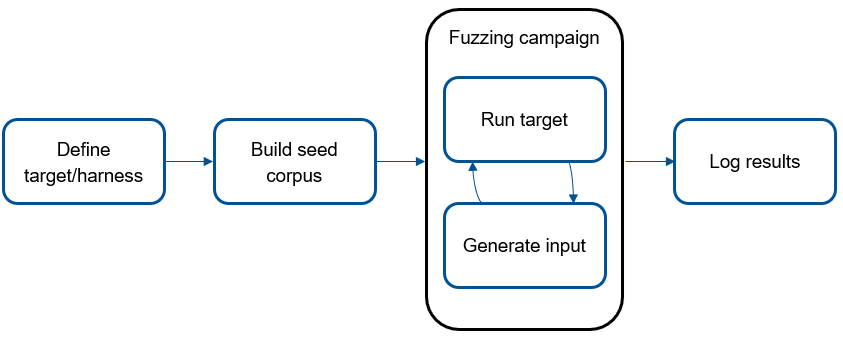
\includegraphics[height=50mm]{figures/fuzzing_steps.png}
    \caption[Fuzzing steps]{Base steps for fuzzing}\label{fig:fuzzing-steps}
\end{figure}

No matter what fuzzer is used, there are a couple of things that are needed to start any fuzzing campaign. Firstly,
the user needs to provide a seed corpus, which is a base set of inputs that the fuzzer will use to generate new
inputs. Secondly, a target program needs to be provided. This may sound simple, but in practice the target will not
always have a friendly entry point, or one that directly accepts input. For instance, the target may be a library,
which will not commonly have a main function. Here, the user first needs to write a small program that will call
some desired parts of the target's code, and then pass the input to it. This is known as a harness.

Fuzzing can be broken down into two main categories, based on the type of target program that is being fuzzed
~\parencite{10.1145/1292414.1292416}. If the target is an open-source program, then the fuzzer is commonly referred 
to as a white-box fuzzer. In this case, the fuzzer has access to the source code, and it can use all inherent information 
to aid in the fuzzing process. For example, the target can be compiled with instrumentation, a technique that adds extra 
flags to the code. These can be used to detect memory corruption, or to provide code coverage information to the fuzzer.
Furthermore, the code coverage can then be used by the fuzzer, to guide the generation of new inputs that are more likely
to reach unexplored code regions.

If the target is a binary, or a closed-source program, then the fuzzer is commonly referred to as a black-box fuzzer.
In this case, the fuzzer doesn't have access to the source code, and so it can't alter the target program at
compile-time. This means that the fuzzer has to have a way of dynamically interpreting the instructions of the target.
A common way to do this is to use an emulator, which can run the target in a virtual environment. This can be taken one
step further, with the fuzzer dynamically adding instrumentation~\parencite{CHEN2018118} after interpreting the source code 
during execution.

The focus of this thesis is on black-box fuzzing. Since binary fuzzing is more difficult than white-box fuzzing, as it loses
some of the directedness that comes from having access to the source code, and being able to compile the target with
instrumentation, it is important to remedy this with other approaches. In the following, we will look at how address
sanitization can be used to improve the effectiveness of binary fuzzing, and how QEMU can be integrated with this
sanitization.


\subsection{QEMU}
QEMU~\parencite{269444} is a machine emulator and virtualizer that can emulate several architectures, on a variety of hosts.
This ability to monitor and control execution in a sandboxed environment, with many different architectures, makes it a
popular choice for fuzzing. For this use case, QEMU is used to run the target application, and it provides the fuzzer
with the ability to dynamically instrument the executed code. Thanks to QEMU being an open-source project, this makes it
easy for fuzzer developers to create their own custom versions of QEMU, tailored to their specific implementation of
a fuzzer~\parencite{257204}. A representation of how QEMU usually interacts with fuzzers can be seen
in~\autoref{fig:qemu-interaction}.

\begin{figure}[htpb]
    \centering
    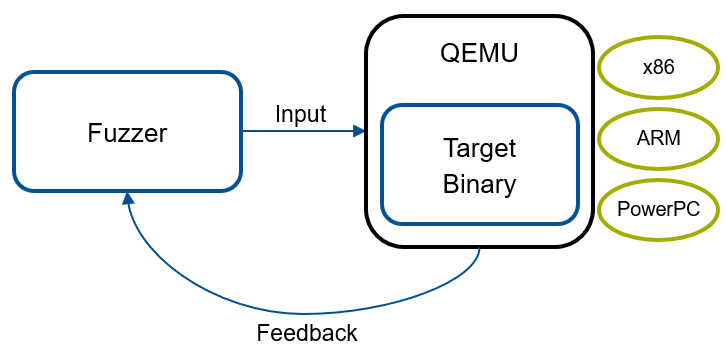
\includegraphics[height=50mm]{figures/qemu_interaction.png}
    \caption[Qemu interaction]{QEMU interaction with fuzzers}\label{fig:qemu-interaction}
\end{figure}

While QEMU is not the only tool of this kind that can be used for fuzzing, there are a number of features that make it 
particularly suitable. Valgrind~\parencite{10.1145/1250734.1250746} and Pin~\parencite{10.1145/1275571.1275600} are two 
other popular tools that offer dynamic binary instrumentation, but they are less versatile in terms of the architectures
that they support. Moreover, QEMU also allows for full-system emulation, which presents the interesting possibility of
full-system fuzzing~\parencite{malmain:hal-04500872}. Another extremely useful feature for fuzzing, specifically
in system mode, is the ability to save and restore the state of the target program, by using the snapshot capabilities
of QEMU.\@ While these snapshots are too slow to be used in a fuzzing loop, they can be used to restore the \ac{VM}, without
having to go through the slow boot phase.

One of the most useful consequences of being able to instrument code, is that it allows for the addition of address
sanitization. This is a technique that adds extra checks to the program, in order to detect memory corruption issues.
Address sanitization comes with a considerable performance penalty, but it is usually a good idea to use it when fuzzing.
In the following section, we will look at how address sanitization can be used to improve the effectiveness of fuzzing, and
discuss how \ac{ASAN} and \ac{QASAN} can be used in combination with QEMU.\@


\subsection{ASAN/QASAN}
\ac{ASAN}~\parencite{10.5555/2342821.2342849} is a memory error detector that can be used to find memory corruption issues in
programs. It was developed by Google, as part of their family of sanitizers~\parencite{43308}
~\parencite{10.1145/1791194.1791203}, and it is now widely used in the industry, also being integrated into LLVM.\@

There are two main components to \ac{ASAN}. The first is the shadow memory. This is a representation of the target
program's memory, where each byte is used to signal whether the 8 corresponding bytes in the actual memory are addressable
or not. A visual representation of this can be seen in~\autoref{fig:asan-shadow-memory}.

\begin{figure}[htpb]
    \centering
    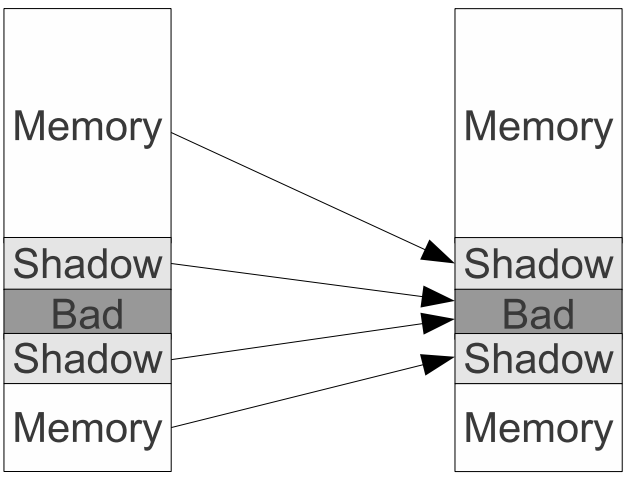
\includegraphics[height=50mm]{figures/asan_shadow_memory.png}
    \caption[ASAN Shadow]{\ac{ASAN} memory mapping~\parencite{10.5555/2342821.2342849}}\label{fig:asan-shadow-memory}
\end{figure}

The second main component of \ac{ASAN} is the instrumentation. This is the part that actually adds the checks to the
target. Every time a memory access is made, the instrumentation will query the shadow memory to see if the bytes that
are being accessed are valid or not. In order for the shadow memory to keep a track of whether or not a part of the
memory is addressable, there is also instrumentation added to the allocation and deallocation functions. This way, the
shadow memory is updated whenever memory is allocated or freed, and queried whenever a write or read is called. One other
important aspect of \ac{ASAN} is that it can also detect out-of-bounds accesses around stack and global objects. This is
done by adding a poisoned `redzone' around these objects, which trigger a crash if they are accessed.


\ac{QASAN}~\parencite{9230171} is an extension of \ac{ASAN}, that is specifically designed to work with QEMU, and to be used
in a fuzzing framework, for black-box fuzzing. The main idea behind \ac{QASAN} is to dynamically add address sanitization
to the target program, by using QEMU to interpret the instructions of the target. The \ac{TCG} feature of QEMU is used to
translate the target's instructions into a form that can be executed on the host. This translation can be leveraged to
add additional instructions, that will perform the \ac{ASAN} checks. A representation of the \ac{QASAN} architecture can be
seen in~\autoref{fig:qasan}.

\begin{figure}[htpb]
    \centering
    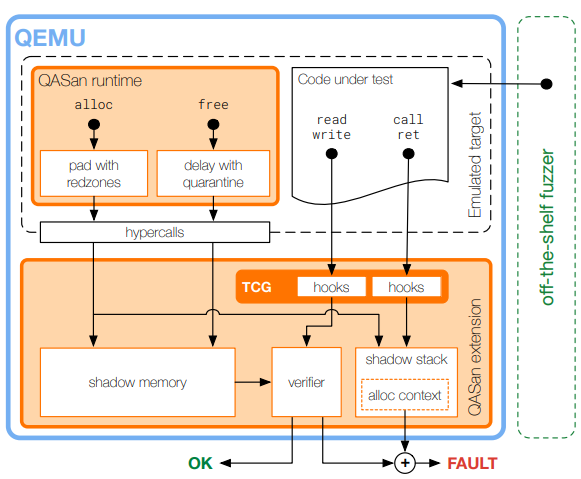
\includegraphics[height=90mm]{figures/qasan.png}
    \caption[QASAN]{\ac{QASAN} architecture~\parencite{9230171}}\label{fig:qasan}
\end{figure}


\section{Motivation}
In software security, memory corruption bugs are a constant source of vulnerabilities. These bugs include buffer overflows,
use-after-free, double-free, and can be exploited by malicious actors, as was the case with the Heartbleed 
bug~\parencite{10.1145/2663716.2663755}. Despite the widespread use of many different tools and techniques to find these bugs,
such as address sanitization and fuzzing, they still remain a problem. Often times it was the wider coding community that
found these bugs, and not the developers themselves. One of the largest obstacles in enabling the community to discover
more bugs, is that in a lot of cases, the source code is not available, only the binary. 

Here, it is important to note that black-box fuzzing is not necessarily slower than white-box fuzzing
~\parencite{electronics12143010}, but it is more difficult to get the same level of coverage, and so it will be slower overall
in finding bugs. Without the ability to compile the target with instrumentation, the fuzzer has much less information at its
disposal with which to generate better inputs. As a result, in the case of binary-only fuzzing, it is much more important to 
increase the speed of the fuzzing campaign, than in standard white-box fuzzing.

As previously discussed, \ac{ASAN}\textbackslash\ac{QASAN} comes with a significant performance penalty. The additional 
bookkeeping that is required to maintain the shadow memory, and the extra checks that are added to the target, slow down 
the fuzzer considerably. However, regardless of whether the fuzzer is running in white-box or black-box mode, it is
usually a good practice to use address sanitization in the fuzzing campaigns. Using \ac{ASAN} for fuzzing can reveal
bugs that would otherwise go unnoticed~\parencite{malmain:hal-04500872}, and it can also provide the fuzzer with better
information about the crash.

In this thesis, the focus will be on improving the performance of binary-only fuzzing with address sanitization. The goal is not
simply to reduce the performance overhead of \ac{QASAN}, but to do so in a way that does not negatively impact the fuzzing
campaigns, by reducing the bugs that are found. The main idea is to give the fuzzer the power to decide dynamically which
parts of the code should be instrumented with sanitization, and which parts shouldn't. This can be done by using different
heuristics and settings, that will be evaluated, to determine which set of these would be the most effective in practice.
% !TeX root = ../main.tex
% Add the above to each chapter to make compiling the PDF easier in some editors.

\chapter{State of the art}\label{chapter:state_of_the_art}
Despite having been around for a few decades, fuzzing has begun to gain a lot more popularity in recent years~\parencite{8371326}.
While the idea of fuzzing may appear simple at its core, there have been so many advancements that have enabled popular fuzzing
frameworks to implement some very interesting optimizations. Some of the main areas that these frameworks often focus
on improving are the following:

\begin{itemize}
    \item \textbf{Input generation}: This component is responsible for generating the input corpus that will be used to
    run the target application. The most basic form of input generation is to simply create random inputs. The next step
    in terms of complexity, is to use more complex algorithm-based approaches, such as bit or byte flipping. Finally,
    most performant fuzzers also take into account the structure of the input data, as well as leverage the knowledge
    provided by coverage data of the target.
    \item \textbf{Corpus management}: Any fuzzing campaign begins with an initial set of seed inputs, generally provided by the
    user. As the campaign progresses, and the fuzzer generates additional inputs, the corpus grows. This is where corpus
    management comes into play, as it falls to the fuzzer to decide which inputs to keep in the corpus, and which to discard.
    This is necessary in order to avoid wasting resources on inputs that are not likely to trigger new code paths, since otherwise
    the corpus would grow to huge sizes. Common heuristics of determining which inputs to keep are based on coverage data, or
    on the performance of the target application when processing the input, in terms of crashes, hangs, execution speed, etc.
    \item \textbf{Coverage data}: Keeping track of the code coverage achieved by target runs is a key component of any 
    modern fuzzer. Firstly, this info can provide the user with relevant statistics about the campaign. Secondly, coverage info
    is perhaps the most important factor in determining the quality of the inputs generated by the fuzzer. Coverage data can
    relate to basic block coverage, edge coverage, function coverage, etc. The goal of the fuzzer is to have reliable coverage
    tracking, while also keeping the overhead of this tracking to a minimum.
    \item \textbf{Instrumentation}: In order to collect coverage data, and to also add additional features like \ac{ASAN},
    the fuzzer needs to add some bits of code to the target, which perform the necessary operations. This is done either
    at compile time, by using special compilers~\parencite{8989335}, or at runtime, by using dynamic binary 
    instrumentation~\parencite{269899}.
\end{itemize}

In the following sections, an overview of some of the most popular fuzzing frameworks, AFL++ and LibAFL, will be provided.
These two frameworks have been chosen because they are well integrated with QEMU, and have solid implementations for the
\ac{QASAN} feature for binary-only fuzzing.


\section{AFL++}
AFL++ is a fork of the original \ac{AFL} coverage-guided fuzzer~\parencite{257204}. The main goal of AFL++ is to

\section{LibAFL}


\section{Current shortcomings}
% !TeX root = ../main.tex
% Add the above to each chapter to make compiling the PDF easier in some editors.

\chapter{Dynamic sanitization}\label{chapter:dynamic_sanitization}

\section{Concept}


\section{Implementation}

\subsection{Block module}

\subsection{Edges module}

\subsection{Comparison of approaches}
% !TeX root = ../main.tex
% Add the above to each chapter to make compiling the PDF easier in some editors.

\chapter{Evaluation}\label{chapter:evaluation}

\section{Setup}

\subsection{Hardware}

\subsection{Fuzzer used}

\subsection{Target programs}

\subsection{Run scripts}


\section{Metrics} % Also discuss best configs using metrics

\subsection{Bugs detected}


\subsection{Execution speed}

% !TeX root = ../main.tex
% Add the above to each chapter to make compiling the PDF easier in some editors.

\chapter{Future work}\label{chapter:future_work}
% Can be combined with what is misssing what can/can't be done better etc.

\section{Fully in-memory bookkeeping}

\section{Dynamic parameter mutation}
% !TeX root = ../main.tex
% Add the above to each chapter to make compiling the PDF easier in some editors.

\chapter{Conclusion}\label{chapter:conclusion}
% TODO: add more chapters here

\appendix{}

\microtypesetup{protrusion=false}

\addchap{Abbreviations}
\begin{acronym}
	\itemsep-.25\baselineskip{}
	\acro{TUM}[TUM]{Technical University of Munich}
	\acro{VM}[VM]{Virtual Machine}
	\acro{ASAN}[ASAN]{Address Sanitizer}
	\acro{QASAN}[QASAN]{QEMU Address Sanitizer}
	\acro{TCG}[TCG]{Tiny Code Generator}
	\acro{AFL}[AFL]{American Fuzzy Lop}
	% TODO: add acronyms
\end{acronym}

\listoffigures{}
\listoftables{}
\microtypesetup{protrusion=true}
\printbibliography{}

\end{document}
